\documentclass[conference]{IEEEtran}

\usepackage[T1]{fontenc}
\usepackage[utf8]{inputenc}
\usepackage{lmodern}
\usepackage{amsmath}
\usepackage{booktabs}
\usepackage{graphicx}
\usepackage{tikz}
\usepackage{xcolor}
\usetikzlibrary{arrows.meta,positioning,shapes.geometric}

\title{A Browser-Based Signalized Intersection Simulator for Transportation Education: Control Logic and Crash-Avoidance Behavior}

\author{
\IEEEauthorblockN{Kun Xie}
\IEEEauthorblockA{
Department of Civil and Environmental Engineering\\
Old Dominion University\\
Norfolk, Virginia, USA\\
\texttt{kxie@odu.edu}
}
}

\begin{document}

\maketitle

\begin{abstract}
This paper presents a browser-based signalized intersection simulator developed for transportation engineering education. The simulator represents a four-leg intersection with one inbound lane per approach, stochastic arrivals, left/through/right turning movements, pedestrian crossings, and a two-phase signal controller with red, green, yellow, and all-red intervals. The model is intended for classroom use rather than field calibration, with emphasis on transparency, responsiveness, and operational interpretation. Particular attention is given to the simulator's control logic and crash-avoidance behavior. Vehicles respond to stop lines, signal indication, leading vehicles, pedestrians, and permissive left-turn conflicts. Pedestrians respond to signal opportunity, nearby vehicles, and in-crosswalk obstructions. A six-scenario evaluation illustrates how changes in turning demand, truck share, pedestrian activity, and directional imbalance affect average delay, queueing, and throughput. The results show especially strong degradation under heavier pedestrian demand and demonstrate that reallocating green time to the dominant east-west phase improves throughput under directional imbalance. The resulting tool supports instruction in queueing, delay, permissive turning, pedestrian interaction, and the relationship between control settings and intersection performance.
\end{abstract}

\begin{IEEEkeywords}
traffic simulation, signalized intersections, transportation education, permissive left turn, pedestrian safety, browser-based simulator
\end{IEEEkeywords}

\section{Introduction}
Traffic engineering courses often introduce signal timing, queueing, and delay through analytical methods before students can observe the resulting operations dynamically. Foundational fixed-time signal timing practice is commonly traced to Webster's classic treatment of signal settings \cite{webster1958}, while modern operational analysis and multimodal performance assessment are typically framed using resources such as the \emph{Highway Capacity Manual} and the \emph{Signal Timing Manual} \cite{hcm2016,stm2015}. While those analytical methods are essential, they do not always convey how traffic streams interact moment by moment at a signalized intersection. A compact visual simulator can bridge that gap by allowing students to modify timing and demand inputs, then immediately observe queue growth, clearance, and conflicts.

The Intersection Simulator described in this paper was developed as a browser-based instructional tool for CEE 370 Transportation Fundamentals. The simulator is intentionally lightweight, but it captures several behaviors that are central to signalized intersection operations:
\begin{itemize}
\item stochastic vehicle arrivals by approach,
\item mixed left, through, and right turning movements,
\item fixed-time two-phase control with yellow and all-red clearance,
\item pedestrian crossings on all approaches,
\item queue and delay reporting in real time, and
\item conflict-sensitive vehicle and pedestrian behavior.
\end{itemize}

The paper focuses especially on two aspects of the model: the control logic governing signal and movement permission, and the crash-avoidance logic that prevents unrealistic overlap among vehicles and pedestrians. In that sense, the simulator is positioned as an instructional bridge between standard traffic engineering references and more detailed microscopic or safety-oriented studies of vehicle and pedestrian interaction \cite{treiber2000,ni2016,zhang2020}. The paper makes three main contributions: it documents a compact browser-based simulator architecture for instruction, formalizes the rule-based control and conflict-avoidance logic used for vehicles and pedestrians, and demonstrates a structured six-scenario evaluation using classroom-friendly performance measures.

\section{System Configuration}
The simulator represents a four-leg intersection with one inbound lane on each approach. Vehicles are animated on lane-based trajectories over a canvas display, while a matching analysis script supports repeated scenario testing. User inputs include:
\begin{itemize}
\item east-west green duration,
\item north-south green duration,
\item yellow duration,
\item all-red duration,
\item approach-specific arrival rates,
\item free-flow speed,
\item left-turn ratio,
\item right-turn ratio,
\item large-vehicle ratio, and
\item simulation speed.
\end{itemize}

The geometric layout includes marked stop lines, crosswalks, and path definitions for through, left-turn, and right-turn movements. Crosswalks and stop bars are encoded directly in the same geometry used by the movement model so that vehicle stopping behavior remains consistent with what is displayed.

\begin{figure}[!t]
\centering
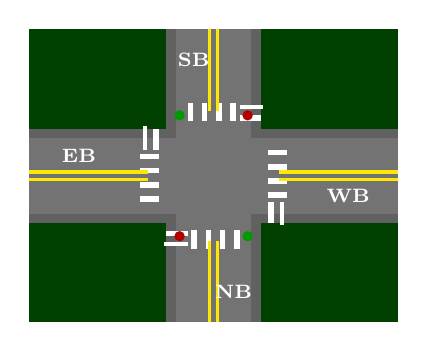
\begin{tikzpicture}[scale=0.6]
  \fill[green!25!black] (-3.9,-3.1) rectangle (3.9,3.1);
  \fill[black!62] (-3.9,-1.0) rectangle (3.9,1.0);
  \fill[black!62] (-1.0,-3.1) rectangle (1.0,3.1);

  \fill[black!55] (-3.9,-0.8) rectangle (3.9,0.8);
  \fill[black!55] (-0.8,-3.1) rectangle (0.8,3.1);

  \draw[white,line width=1.4pt] (-1.45,0.55) -- (-1.45,1.05);
  \draw[white,line width=1.4pt] (1.45,-0.55) -- (1.45,-1.05);
  \draw[white,line width=1.4pt] (-0.55,-1.45) -- (-1.05,-1.45);
  \draw[white,line width=1.4pt] (0.55,1.45) -- (1.05,1.45);

  \foreach \y in {-0.55,-0.25,0.05,0.35} {
    \fill[white!85] (-1.55,\y) rectangle (-1.15,\y+0.12);
    \fill[white!85] (1.15,-\y-0.12) rectangle (1.55,-\y);
  }
  \foreach \x in {-0.55,-0.25,0.05,0.35} {
    \fill[white!85] (\x,1.15) rectangle (\x+0.12,1.55);
    \fill[white!85] (-\x-0.12,-1.55) rectangle (-\x,-1.15);
  }

  \draw[yellow!90!orange,line width=1.2pt] (-3.9,-0.08) -- (-1.38,-0.08);
  \draw[yellow!90!orange,line width=1.2pt] (1.38,-0.08) -- (3.9,-0.08);
  \draw[yellow!90!orange,line width=1.2pt] (-3.9,0.08) -- (-1.38,0.08);
  \draw[yellow!90!orange,line width=1.2pt] (1.38,0.08) -- (3.9,0.08);
  \draw[yellow!90!orange,line width=1.2pt] (-0.08,-3.1) -- (-0.08,-1.38);
  \draw[yellow!90!orange,line width=1.2pt] (-0.08,1.38) -- (-0.08,3.1);
  \draw[yellow!90!orange,line width=1.2pt] (0.08,-3.1) -- (0.08,-1.38);
  \draw[yellow!90!orange,line width=1.2pt] (0.08,1.38) -- (0.08,3.1);

  \draw[white,line width=2pt] (-1.22,0.55) -- (-1.22,1.0);
  \draw[white,line width=2pt] (1.22,-0.55) -- (1.22,-1.0);
  \draw[white,line width=2pt] (-0.55,-1.22) -- (-1.0,-1.22);
  \draw[white,line width=2pt] (0.55,1.22) -- (1.0,1.22);

  \fill[green!60!black] (-0.72,1.28) circle (0.11);
  \fill[red!70!black] (0.72,1.28) circle (0.11);
  \fill[red!70!black] (-0.72,-1.28) circle (0.11);
  \fill[green!60!black] (0.72,-1.28) circle (0.11);

  \node[white,font=\scriptsize\bfseries] at (-2.85,0.42) {EB};
  \node[white,font=\scriptsize\bfseries] at (2.85,-0.42) {WB};
  \node[white,font=\scriptsize\bfseries] at (-0.42,2.45) {SB};
  \node[white,font=\scriptsize\bfseries] at (0.42,-2.45) {NB};
\end{tikzpicture}
\caption{Schematic intersection view used by the simulator, showing a four-leg layout with stop lines, crosswalks, lane-based approaches, and two-phase signal control.}
\label{fig:intersection_view}
\end{figure}

Figure~\ref{fig:intersection_view} summarizes the instructional geometry represented in the simulator. Although simplified to one inbound lane per approach, the view retains the control and conflict elements needed to illustrate queueing, clearance, turning interactions, and pedestrian crossings.

\begin{figure}[!t]
\centering
\resizebox{\columnwidth}{!}{%
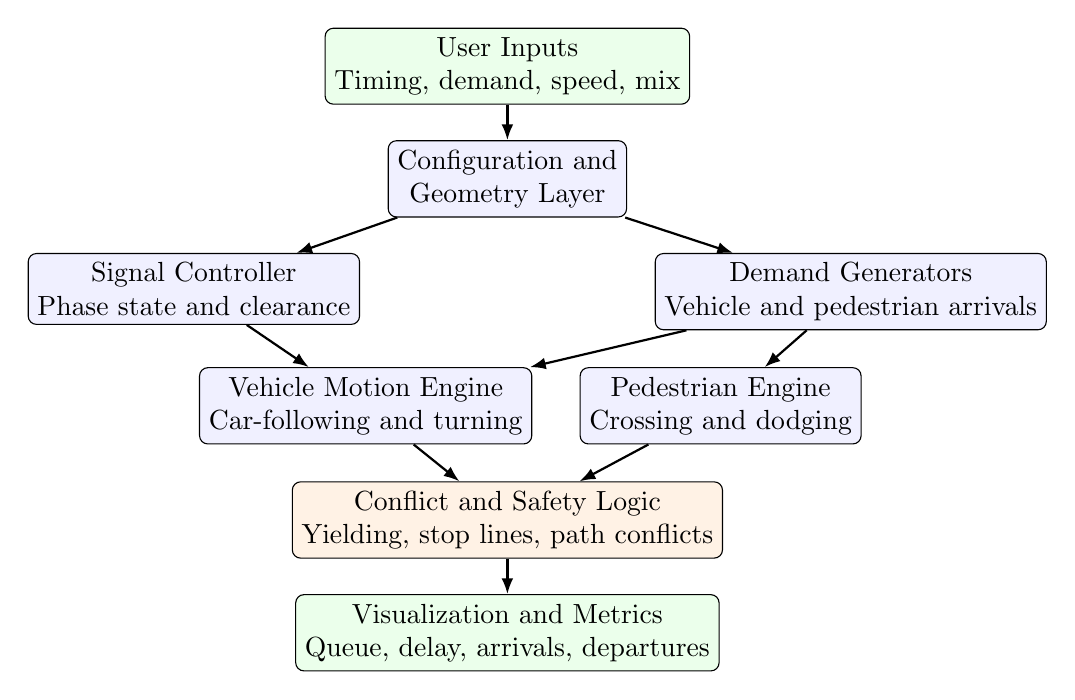
\begin{tikzpicture}[
  node distance=0.45cm and 0.35cm,
  module/.style={draw, rounded corners=3pt, align=center, minimum width=2.85cm, minimum height=0.8cm, fill=blue!6},
  io/.style={draw, rounded corners=3pt, align=center, minimum width=2.85cm, minimum height=0.8cm, fill=green!8},
  logic/.style={draw, rounded corners=3pt, align=center, minimum width=2.85cm, minimum height=0.8cm, fill=orange!10},
  arr/.style={-{Latex[length=2mm]}, thick}
]
  \node[io] (inputs) {User Inputs\\Timing, demand, speed, mix};
  \node[module, below=of inputs] (config) {Configuration and\\Geometry Layer};
  \node[module, below left=of config] (signal) {Signal Controller\\Phase state and clearance};
  \node[module, below right=of config] (demand) {Demand Generators\\Vehicle and pedestrian arrivals};
  \node[module, below=of config, yshift=-1.45cm, xshift=-1.8cm] (veh) {Vehicle Motion Engine\\Car-following and turning};
  \node[module, right=0.6cm of veh] (ped) {Pedestrian Engine\\Crossing and dodging};
  \node[logic, below=of config, yshift=-2.9cm] (safety) {Conflict and Safety Logic\\Yielding, stop lines, path conflicts};
  \node[io, below=of safety] (outputs) {Visualization and Metrics\\Queue, delay, arrivals, departures};

  \draw[arr] (inputs) -- (config);
  \draw[arr] (config) -- (signal);
  \draw[arr] (config) -- (demand);
  \draw[arr] (signal) -- (veh);
  \draw[arr] (demand) -- (veh);
  \draw[arr] (demand) -- (ped);
  \draw[arr] (veh) -- (safety);
  \draw[arr] (ped) -- (safety);
  \draw[arr] (safety) -- (outputs);
\end{tikzpicture}
}
\caption{Framework of the simulator's key modules. The model combines configuration, fixed-time control, stochastic demand generation, vehicle and pedestrian behavior engines, conflict handling, and live performance reporting.}
\label{fig:framework}
\end{figure}

Figure~\ref{fig:framework} shows the key module structure. Configuration data feeds both the signal controller and the demand generators, while vehicle and pedestrian behavior are coordinated through shared conflict and safety logic before being passed to the visualization and metric layers.

\section{Signal Control Logic}
\subsection{Phase Structure}
The simulator uses a fixed two-phase sequence:
\begin{enumerate}
\item east-west green,
\item east-west yellow,
\item east-west all-red,
\item north-south green,
\item north-south yellow,
\item north-south all-red.
\end{enumerate}

Each approach is assigned to either the east-west or north-south phase group. The current state determines the active service interval, and elapsed time is compared against the configured duration for the current state. This allows students to observe how green splits and clearance intervals influence queue dynamics and throughput. The structure is intentionally simple, but it follows the broad fixed-time timing concepts described in standard signal timing references \cite{webster1958,stm2015}.

\subsection{Movement Permission}
A vehicle is permitted to proceed when its approach belongs to the active green phase. In addition, the simulator includes a targeted yellow-clearance rule for permissive left-turn vehicles. At the transition from green to yellow, the lead left-turn vehicle on each active approach may be tagged for completion during the yellow interval. This prevents a waiting permissive left-turn vehicle from blocking the queue unnecessarily while avoiding the unrealistic behavior of releasing multiple queued vehicles during yellow.

Algorithm~\ref{alg:signal_permission} summarizes the core phase-update and movement-permission logic used by the simulator.

\begin{figure}[!t]
\centering
\fbox{%
\begin{minipage}{0.90\columnwidth}
\scriptsize
\textbf{Algorithm 1. Signal update and vehicle permission}
\begin{tabbing}
\hspace{0.8em}\=\hspace{0.8em}\=\hspace{0.8em}\=\kill
\textbf{Input:} current signal state, elapsed time, phase durations, approach queues\\
\textbf{If} elapsed time exceeds current state duration:\\
\> \textbf{if} state = EW-Green:\\
\>\> tag lead left-turn vehicles on active EW approaches\\
\>\> state $\leftarrow$ EW-Yellow\\
\> \textbf{else if} state = EW-Yellow:\\
\>\> clear yellow left-turn tags\\
\>\> state $\leftarrow$ EW-All-Red\\
\> \textbf{else if} state = EW-All-Red:\\
\>\> state $\leftarrow$ NS-Green\\
\> \textbf{else if} state = NS-Green:\\
\>\> tag lead left-turn vehicles on active NS approaches\\
\>\> state $\leftarrow$ NS-Yellow\\
\> \textbf{else if} state = NS-Yellow:\\
\>\> clear yellow left-turn tags\\
\>\> state $\leftarrow$ NS-All-Red\\
\> \textbf{else}:\\
\>\> state $\leftarrow$ EW-Green\\
\textbf{For each} vehicle approaching the stop line:\\
\> \textbf{if} its phase group has green, vehicle is permitted\\
\> \textbf{else if} state is yellow \textbf{and} vehicle is tagged\\
\>\> lead left-turner, vehicle is permitted\\
\> \textbf{else} vehicle must stop at the stop line\\
\end{tabbing}
\end{minipage}%
}
\caption{Pseudocode for phase progression and movement permission.}
\label{alg:signal_permission}
\end{figure}

\subsection{Pedestrian Release Logic}
Pedestrian demand is generated stochastically and stored as pending requests. A pedestrian may begin crossing only when the corresponding vehicle approach is not green and the entry area is comfortable, meaning no nearby lead vehicle is still moving aggressively into the crosswalk zone. This provides a simplified but instructionally useful representation of pedestrian opportunity under signal control and reflects the multimodal emphasis recommended in contemporary signal timing guidance \cite{stm2015}.

\section{Vehicle Motion Model}
\subsection{Arrival and Movement Generation}
Vehicles are generated on each approach using exponentially distributed headways based on user-defined hourly arrival rates. Upon creation, each vehicle is assigned a movement type and desired speed. Vehicle size may vary to represent a mixture of passenger vehicles and larger vehicles.

\subsection{Car-Following}
Approach vehicles use a simplified Intelligent Driver Model style acceleration rule. For each vehicle, the simulation identifies the most restrictive lead object, which may be:
\begin{itemize}
\item the preceding vehicle in the same approach queue,
\item a same-approach vehicle that has just entered the intersection,
\item a stationary stop-line control induced by the signal,
\item a stop condition caused by a pedestrian conflict, or
\item a stop condition caused by a permissive turning conflict.
\end{itemize}

This structure allows vehicles to decelerate smoothly into stop conditions rather than relying on abrupt position clipping alone. Although simplified for classroom use, the formulation is directly inspired by the Intelligent Driver Model literature \cite{treiber2000}.

\subsection{Queue Measurement}
Queue count is estimated from vehicles that are either stopped near the stop line or trapped behind such vehicles with sufficiently small following gaps. This produces a real-time queue measure suitable for classroom comparison of timing scenarios. In the analysis script, average queue is computed as the time-integrated queue count divided by simulation time, while maximum queue is the largest instantaneous queue observed during a replication.

\section{Crash-Avoidance Behavior for Vehicles}
Crash avoidance in the simulator is conflict-based. Instead of resolving overlap after it occurs, the model forecasts potential conflicts and converts them into temporary control points or progress limits. This emphasis on interaction and conflict is consistent with broader safety research that treats surrogate conflicts as a useful lens for analyzing road-user behavior when collision events are sparse \cite{ni2016,zhang2020}.

\subsection{Rear-End Avoidance}
Vehicles maintain longitudinal separation by tracking the front-to-rear gap to the leader in the same approach queue. The same separation logic is extended to the entry area of the intersection so that a following vehicle does not run into a same-approach vehicle that has only partially advanced into the intersection.

\subsection{Stop-Line and Signal Compliance}
When a movement is not permitted by the current signal state, the stop line acts as a stationary lead object. This keeps vehicles from encroaching into the intersection during red or all-red conditions and ties the visible stop position to the same control geometry used in the motion model.

\subsection{Permissive Left Turns Against Opposing Through Traffic}
For left-turn vehicles, the simulator computes a conflict profile by locating where the left-turn path intersects the opposing through path. If an opposing through vehicle is close enough to that conflict point, the left-turn vehicle yields before entering. If the left-turn vehicle has already entered the intersection, it may continue to wait inside the intersection until the opposing stream clears. This models the common permissive behavior in which drivers accept a gap only after encroaching into the intersection.

\subsection{Permissive Left Turns Against Opposing Right Turns}
The model also checks for a shared receiving lane conflict between permissive left turns and opposing right turns. The simulator identifies where the left-turn path and opposing right-turn path converge into the same outbound lane and uses that location to define another yielding region. As a result, left-turn vehicles can be held either at the stop line or inside the intersection if an opposing right-turn vehicle would occupy the receiving lane first.

\subsection{In-Intersection Route Separation}
Once vehicles are inside the intersection, they are grouped by route and ordered by progress along that route. Followers are prevented from exceeding the leader's progress minus a minimum spacing threshold. This reduces the likelihood of overlap among vehicles taking the same path and improves visual consistency.

\section{Crash-Avoidance Behavior for Pedestrians}
\subsection{Crosswalk Entry Screening}
Pedestrians are not released automatically at the instant vehicle green ends. Instead, the model checks whether the lead vehicle near the stop line is sufficiently far back or nearly stopped before allowing a crossing to begin. This prevents pedestrians from spawning directly into a hazardous situation.

\subsection{Crosswalk Occupancy and Lateral Offsets}
Pedestrians are assigned lateral offsets within the crosswalk so that multiple pedestrians can occupy the crossing simultaneously without collapsing into the same centerline. Entry spacing rules reduce immediate overlap near the curb line.

\subsection{Obstacle Avoidance While Crossing}
Each pedestrian evaluates the next desired position along the crosswalk. If a vehicle blocks that projected position, the pedestrian searches a set of lateral dodge candidates. When a safe lateral offset is found, the pedestrian continues with a sidestep-like adjustment. If no safe option is available, the pedestrian slows or stops. This creates a simple local avoidance behavior that is visually intuitive and educationally useful.

\subsection{Vehicle Yielding to Pedestrians}
Vehicles inside the intersection also check whether a pedestrian lies sufficiently close to their projected path. If so, the vehicle receives a stop progress ahead of the conflict point and yields until the pedestrian clears. This treats pedestrian safety as an active control input to vehicle behavior.

Algorithm~\ref{alg:conflict_update} summarizes the key conflict-aware crash-avoidance logic for a vehicle near or within the intersection.

\begin{figure}[!t]
\centering
\fbox{%
\begin{minipage}{0.90\columnwidth}
\scriptsize
\textbf{Algorithm 2. Conflict-aware vehicle update}
\begin{tabbing}
\hspace{0.8em}\=\hspace{0.8em}\=\hspace{0.8em}\=\kill
\textbf{Input:} vehicle $i$, nearby vehicles, signal state, pedestrians\\
\textbf{Initialize} lead object $\leftarrow$ none\\
\textbf{If} a same-approach leader exists:\\
\> set lead object from front-to-rear spacing and leader speed\\
\textbf{If} signal is not permissive \textbf{or} crosswalk is occupied:\\
\> set lead object to stop line if more restrictive\\
\textbf{If} vehicle $i$ is a left-turner and opposing through conflict exists:\\
\> set lead object to left-turn yield point if more restrictive\\
\textbf{If} vehicle $i$ is a left-turner and opposing right-turn conflict exists:\\
\> set lead object to shared-lane yield point if more restrictive\\
\textbf{Compute} acceleration from the most restrictive lead object\\
\textbf{Advance} vehicle toward stop line or into the intersection\\
\textbf{If} vehicle is inside the intersection:\\
\> locate nearest pedestrian conflict along planned path\\
\> limit progress to the earliest active stop progress\\
\> enforce route-based spacing behind any same-route leader\\
\textbf{If} path is completed:\\
\> record trip completion and delay\\
\end{tabbing}
\end{minipage}%
}
\caption{Pseudocode for conflict-aware crash-avoidance behavior.}
\label{alg:conflict_update}
\end{figure}

\section{Scenario Evaluation and Results}
The simulator can be used to organize a multi-scenario classroom experiment around a consistent baseline. Table~\ref{tab:scenarios} defines six scenarios centered on the default control settings in the browser interface: 30~s east-west green, 3~s yellow, 2~s all-red, 30~s north-south green, 300~veh/h on each approach, 100~ped/h total crossing demand, 30~mph desired speed, 5\% left turns, 5\% right turns, and 5\% large vehicles. The reported measures of interest remain classroom-oriented operational summaries rather than formal \emph{Highway Capacity Manual} outputs, but they correspond to familiar concepts such as delay, queueing, and throughput \cite{hcm2016}.

\begin{table*}[!t]
\caption{Scenario Set for Comparative Experiments}
\label{tab:scenarios}
\centering
\footnotesize
\setlength{\tabcolsep}{4pt}
\begin{tabular}{p{0.85cm} p{3.7cm} p{2.0cm} p{2.9cm} p{2.9cm} p{1.45cm}}
\toprule
ID & Scenario Focus & Signal Timing (EW-Y-AR-NS) & Vehicle Demand (veh/h) & Special Setting Changes & Intended Emphasis \\
\midrule
S1 & Baseline default settings & 30-3-2-30 & W/E/N/S: 300/300/300/300 & Left turn 5\%, right turn 5\%, trucks 5\%, pedestrians 100/h & Reference operating condition \\

S2 & Higher left-turn activity & 30-3-2-30 & W/E/N/S: 300/300/300/300 & Left-turn ratio increased to 30\% & Effect of turning conflicts and permissive left-turn delay \\

S3 & Higher truck proportion & 30-3-2-30 & W/E/N/S: 300/300/300/300 & Large-vehicle ratio increased to 30\% & Effect of heavier vehicles on discharge, spacing, and queue growth \\

S4 & Higher pedestrian demand & 30-3-2-30 & W/E/N/S: 300/300/300/300 & Pedestrian volume increased to 500/h total & Interaction between crosswalk activity and vehicle progression \\

S5 & Heavier east-west demand with unchanged timing & 30-3-2-30 & W/E/N/S: 600/600/300/300 & Other settings remain at baseline & Sensitivity to directional demand imbalance \\

S6 & Heavier east-west demand with retiming & 40-3-2-20 & W/E/N/S: 600/600/300/300 & Other settings remain at baseline & Operational benefit of reallocating green to the dominant phase \\
\bottomrule
\end{tabular}
\end{table*}

The six scenarios are intended to support a structured comparison across geometry-invariant but behaviorally distinct operating conditions. Scenarios S2--S4 isolate one behavioral input at a time relative to the baseline, while Scenarios S5 and S6 form a paired experiment on directional demand imbalance and signal retiming.

Each scenario was evaluated with the companion analysis script using 10 replications of 1200~s per replication. Delay was computed as completed trip time minus nominal free-flow travel time, average queue was measured from the time-integrated queue count, and maximum queue was the largest instantaneous queue observed in a replication. Table~\ref{tab:scenario_metrics} summarizes the mean results.

The results are consistent with the intended instructional contrasts. Increasing the left-turn share from 5\% to 30\% increases average delay from 36.3~s/veh to 45.9~s/veh and average queue from 5.9 to 8.8~veh because more vehicles must wait for permissive gaps. Raising the truck proportion to 30\% produces a milder degradation, increasing delay to 37.1~s/veh. The strongest deterioration occurs under the 500~ped/h scenario, where pedestrian interaction raises average delay to 60.9~s/veh and average queue to 12.6~veh. Under heavier east-west demand, retiming the signal from 30-3-2-30 to 40-3-2-20 reduces average delay from 53.5~s/veh to 51.1~s/veh and improves throughput from 1319.4 to 1446.0~veh/h. However, the mean maximum queue remains high in S6, indicating that retiming improves overall service while still allowing short-lived peak queues under unbalanced demand.

\begin{table}[!t]
\caption{Scenario Performance Metrics}
\label{tab:scenario_metrics}
\centering
\footnotesize
\begin{tabular}{ccccc}
\toprule
ID & Avg. Delay & Avg. Queue & Max Queue & Throughput \\
 & (s/veh) & (veh) & (veh) & (veh/h) \\
\midrule
S1 & 36.3 & 5.9 & 19.5 & 1100.4 \\
S2 & 45.9 & 8.8 & 23.4 & 1117.8 \\
S3 & 37.1 & 6.0 & 17.7 & 1107.0 \\
S4 & 60.9 & 12.6 & 31.5 & 1026.0 \\
S5 & 53.5 & 13.2 & 28.6 & 1319.4 \\
S6 & 51.1 & 13.1 & 33.0 & 1446.0 \\
\bottomrule
\end{tabular}
\end{table}

\section{Educational Use}
The simulator supports several classroom objectives:
\begin{itemize}
\item demonstrating the effect of green splits on queue growth and dissipation,
\item showing how random arrivals create variability around average demand,
\item illustrating why permissive left turns can produce large delays,
\item discussing pedestrian influence on intersection operations, and
\item comparing alternative timing plans without requiring specialized software.
\end{itemize}

Because the logic is compact and visible in code, the simulator is also appropriate for introductory computing exercises in transportation engineering.

\section{Limitations and Future Work}
The current version is intentionally simplified. It uses one inbound lane per approach, fixed-time control, stylized driver behavior, and rule-based pedestrian logic. It is best understood as a teaching simulator rather than a field-validated operational model.

Future extensions could include:
\begin{itemize}
\item protected or protected-permissive left-turn phasing,
\item multiple inbound lanes and lane assignment,
\item approach-specific turning proportions,
\item explicit pedestrian signal indications,
\item richer safety surrogate measures, and
\item automated scenario reporting for classroom assignments.
\end{itemize}

\section{Conclusion}
The Intersection Simulator provides a compact and accessible platform for teaching signalized intersection operations. Its two-phase controller, stochastic arrivals, car-following logic, permissive turning rules, pedestrian interactions, and conflict-based crash-avoidance behavior allow students to connect traffic engineering theory with dynamic system behavior. The scenario study further shows that the tool produces interpretable responses to changes in turning demand, truck share, pedestrian activity, and green allocation. Although simplified, the simulator is rich enough to support meaningful discussion of control, safety, delay, and operational tradeoffs in a classroom setting.

\begin{thebibliography}{00}

\bibitem{webster1958}
F.~V.~Webster, \emph{Traffic Signal Settings}, Road Research Laboratory, Road Research Technical Paper No.~39. London, U.K.: H.M. Stationery Office, 1958.

\bibitem{stm2015}
National Academies of Sciences, Engineering, and Medicine, \emph{Signal Timing Manual -- Second Edition}. Washington, DC, USA: The National Academies Press, 2015, doi: 10.17226/22097.

\bibitem{hcm2016}
Transportation Research Board, \emph{Highway Capacity Manual 6th Edition: A Guide for Multimodal Mobility Analysis}. Washington, DC, USA: The National Academies Press, 2016, doi: 10.17226/24798.

\bibitem{treiber2000}
M.~Treiber, A.~Hennecke, and D.~Helbing, ``Congested traffic states in empirical observations and microscopic simulations,'' \emph{Physical Review E}, vol.~62, no.~2, pp.~1805--1824, 2000, doi: 10.1103/PhysRevE.62.1805.

\bibitem{ni2016}
Y.~Ni, M.~Wang, J.~Sun, and K.~Li, ``Evaluation of pedestrian safety at intersections: A theoretical framework based on pedestrian-vehicle interaction patterns,'' \emph{Accident Analysis \& Prevention}, vol.~96, pp.~118--129, 2016, doi: 10.1016/j.aap.2016.07.030.

\bibitem{zhang2020}
S.~Zhang, M.~Abdel-Aty, Q.~Cai, P.~Li, and J.~Ugan, ``Prediction of pedestrian-vehicle conflicts at signalized intersections based on long short-term memory neural network,'' \emph{Accident Analysis \& Prevention}, vol.~148, Art.~no.~105799, 2020, doi: 10.1016/j.aap.2020.105799.

\end{thebibliography}

\end{document}
